\documentclass[../main.tex]{subfiles}
\graphicspath{{\subfix{../images/}}}
\begin{document}
\subsection{Conditional Probability}
\begin{definition} Given $B\in\mathcal{F}$ an event with $\mathbb{P}(B)>0$ then we define the conditional probability measure - 
\[
    \mathbb{P}_B(A)=\mathbb{P}(A\mid B)=\frac{\mathbb{P}(A\cap B)}{\mathbb{P}(B)}
\]
\end{definition}
Formally this moves us to a know probability space - instead of $(\Omega,\mathcal{F},\mathbb{P})$ we now have $(B,\mathcal{F}\mid_{B}, \mathbb{P}_B)$. \\\\
We can now use this to also consider density functions for a pair of random variables (X,Y) and have $f_Y(b)\cdot f_{X\mid Y=b} = f_{X,Y}(a,b)$. \\\\
\begin{example} Take $X\sim\text{Exp}(\lambda)$, meaning $f_X(t)=\lambda e^{-\lambda t}$. Consider the event $(X-a\leq b\mid X>a)$. This is - 
\[\mathbb{P}(X\leq a+b\mid X>a) = \frac{\mathbb{P}(X\leq a+b, X>a)}{\mathbb{P}(X>a)} = \frac{\int_a^{a+b} \lambda e^{-\lambda t }dt}{\int_a^\infty \lambda e^{-\lambda t }dt}=\]\[=\frac{-e^{-\lambda t}\mid_a^{a+b}}{-e^{-\lambda t}\mid_a^\infty} =\dots=1-e^{-\lambda b} = \mathbb{P}(X\leq b)\]
This is called the memorylessness characteristic of the exponential distribution. \end{example}
\begin{definition} For a discrete random variable X we define the expected value of X to be - $\mathbb{E}[X] = \sum_a a\mathbb{P}(X=a)$. 
For a continuous random variable the expected value to be - $\mathbb{E}[X]=\int_{\mathbb{R}} tf(t) dt$. \end{definition}
\begin{example} Take the binomial distribution $X\sim\text{Bin}(n,p)$. There are many ways to calculate the expected value, it can be done by hand but the more pleasant way of doing this is by using the linearity of the expected value - $\mathbb{E}[X+Y] = \mathbb{E}[X]+\mathbb{E}[Y]$ for any 2 random variables X and Y, and by noticing that the binomial distribution is a sum of n bernoulli experiments $\{X_i\}_{i=1}^n$ each with expected value p and therefore - 
\[\overline{\underline{\mathbb{E}\left[X\right]}} = \mathbb{E}[\sum_{i=1}^n X_i] = \sum_{i=1}^n\mathbb{E}[X_i] = \sum_{i=1}^n p = \overline{\underline{np}}\]
\end{example}
\begin{claim} 
The law of returning expected values is that for any 2 random variables X,Y we have - $\mathbb{E}[Y]=\mathbb{E}[\mathbb{E}[Y\mid X]]$. \end{claim}
\begin{proof}
For this we need to notice that $Y\mid X$ is a function such that every $b\in\mathbb{R}$ maps to the random variable $Y\mid X=b$ and we can ask what it's expected value at each $b\in\mathbb{R}$. The function $\mathbb{E}[Y\mid X]$ does exactly that - for every $b\in\mathbb{R}$ it returns the value $\mathbb{E}[Y\mid X=b]$. Now the claim is that the expected value of $\mathbb{E}[Y\mid X]$ is just $\mathbb{E}[Y]$. 
\end{proof}
\newpage 
\begin{example} Take a school of kids - the sample space is
the the set of all the kids in the school. Y measures the height of a child, and X says what class the child is in. What this tells us is that averaging per class and then over all of the classes is similar to averaging over all of the kids in the school at once. \end{example}
\begin{example} Flip a fair coin until you get "tails", and then toss a fair die the number of times we have tossed "heads" and sum over all of the rolls. \end{example}
We can then take $N\sim\text{Geo}(\frac{1}{2})$, and $X_i\sim U(\{1,2,3,4,5,6\})$ and finally take $Y=\sum_{i=1}^N X_i$. \\\\ Using the previous claim to see that
\[
    \overline{\underline{\mathbb{E}[Y]}} = \mathbb{E}[\mathbb{E}[Y\mid N]] = \mathbb{E}[\mathbb{E}[X_1 \mid N]+\mathbb{E}[X_2 \mid N]+\dots + \mathbb{E}[X_N \mid N]] = 
\]
\[
    =\mathbb{E}[\mathbb{E}[X_1]+\dots+\mathbb{E}[X_N]] = \mathbb{E}[N]\mathbb{E}[X_i] = \frac{7}{2}\cdot 2 = \overline{\underline{7}}
\]
\begin{definition} For a random variable X we can define it's variance in the following way -
\[
    \text{Var}(X) = \mathbb{E}[(X-\mathbb{E}[X])^2] = \mathbb{E}[X^2]-\mathbb{E}[X]^2 
\]
\end{definition}
We can see the following characteristics quite easily - \\\\
- $\text{Var}(X)\geq 0$. \\\\
- For all $a\in\mathbb{R}$ we have $\text{Var}(X+a)=\text{Var}(X)$, and $\text{Var}(a\cdot X)=a^2 \text{Var}(X)$. \\\\
\begin{claim} The law of total variance says that -
\begin{center}
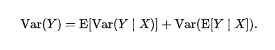
\includegraphics{images/Stat_Theory_Fourth_Image.png}
\end{center}
\end{claim}
\newpage
\subsection{Sufficient Statistics Part 1}
Denote $\bar{y} = (y_1,\dots,y_n)$ to be a sample (a realization) from a random vector $\bar{Y}=(Y_1,\dots,Y_n)$ with some distribution $f_Y(\bar{y})$. We will assume that Y comes from a family of distributions $\mathcal{G}$, which is characterized by a vector of parameters $\bar{\theta}\in\Theta$ where $\Theta$ is the parameter space.  \\\\
Additionally we will also assume that $Y_1,\dots,Y_n$ are i.i.d. from some distribution $f_\theta(y)$ from a family $\mathcal{G}_{\theta}$ for $\theta\in\Theta$.
\begin{example}
\label{Bernoulli}
In a hospital we record the distribution of births - whether they are male (M) or female (F). Let's say this comes out to be - \\\\
(F,M,F,F,M,M,F,M,F,F,F,F,M,M,F,F,F,M,M,F). \\\\
We can now define $Y_i$ to be the indicator function that tells us that the i-th birth was a female. It is natural to assume that $Y_i\sim \text{Ber}(p)$ for some $p\in(0,1)$ i.i.d. So our parameter space is $\Theta = (0,1)$. \end{example}
\begin{example} Someone wants to see how much codeine there is in a pill for headache relief, she purchases 5 pills. On the packaging it says that the amount of codeine in a pill is 200 mg. In the ones she checks at home she observes the following measurements - \\\\
(200.3,195.0,192.4,201.2,190.1) \\\\
A model that fits these measurements could be the normal distribution - $Y_i=\mu+\epsilon_i$ where $\epsilon_i$ are i.i.d. $\mathcal{N}(0,\sigma^2)$. She wants to know what $\mu,\sigma^2$ are most likely to be. \end{example}
Therefore the first task should be the likelihood measurements - \\\\
- From example 2.5, is the probability for a female child $\frac{12}{20}$? \\\\
- The average measurement that she measures in example 2.6 is 196.6 mg, and this is different from what the package says. Is the package "lying"?
\newpage
\subsection{Likelihood:} Given a sample $y=(y_1,\dots,y_n)$ that is a realization of the distribution $Y=(Y_1,\dots,Y_n)$ with distribution $f_\theta(y)$ for $\theta\in\Theta$. \\
Now assume that Y is a discrete random variable, what is the probability to sample y?
\[
    \mathbb{P}_{\theta}(Y_1=y_1,\dots,Y_n=y_n)
\]
\begin{definition} The likelihood function is $L(\theta;y):=\mathbb{P}_\theta(Y=y)$. We consider $\theta_1$ to be a more likely parameter than $\theta_2$ if $L(\theta_1;y)>L(\theta_2;y)$.\end{definition}
If the $Y_i$ are i.i.d. then we have the following result - 
\[
    L(\theta;y) = \prod _{i=1}^n \mathbb{P}_\theta(Y_i=y_i)
\]
For example for example 2.5 we have - 
\[
    L(p;y)=p^{y_1}(1-p)^{1-y_1}\cdots p^{y_n}(1-p)^{1-y_n} = p^{\sum_i y_i}(1-p)^{n-\sum_i y_i}
\]
We can now look at different values of p and compare to see what parameters are more or less likely.
\\\\
Notice that we have defined this for discrete Y, now assume Y is continuous with density function $f_\theta(y)$. The likelihood function is now defined to be - $L(\theta,y)=f_\theta(y)$. Now we lose the exact probabilities but we are still able to compare for different $\theta$'s. As from before we have that for i.i.d. $y_1,\dots,y_n$ - 
\[
    L(\theta;y)=\prod_{i=1}^n f_\theta(y_i)
\]
For example 2.6 we can therefore have - 
\[
    L(\mu,\sigma;y)=\prod_{i=1}^5 \frac{1}{\sqrt{2\pi}\sigma}e^{-\frac{1}{2}(\frac{y_i-\mu}{\sigma})^2}
\]
\end{document}
